% !TeX document-id = {1c0b4298-276a-4038-8e08-c4a1f4846da7}
% !TeX TXS-program:bibliography = txs:///biber
\documentclass[10pt,a4paper]{article}
\usepackage[T1]{fontenc}
\usepackage{graphicx}
\usepackage{mathtools}
\usepackage{amssymb}
\usepackage{amsthm}
\usepackage{thmtools}
\usepackage{xcolor}
\usepackage{nameref}
\usepackage{hyperref}
\usepackage{color}
\usepackage{float}

\usepackage[
backend=biber,
style=authoryear,
natbib=true
]{biblatex}
\addbibresource{../bibliography.bib}


\title{\large EAE1223: Econometria III}
\author{\normalsize Exercícios sobre a metodologia de Box-Jenkins}
\date{}
\begin{document}
	\maketitle
	\paragraph{Parte 1}
	
	\begin{enumerate} 
		\item[1] Observando a FAC e FACP, assinale qual processo é mais provável de ter gerado os dados:
		
		\begin{figure}[H]
			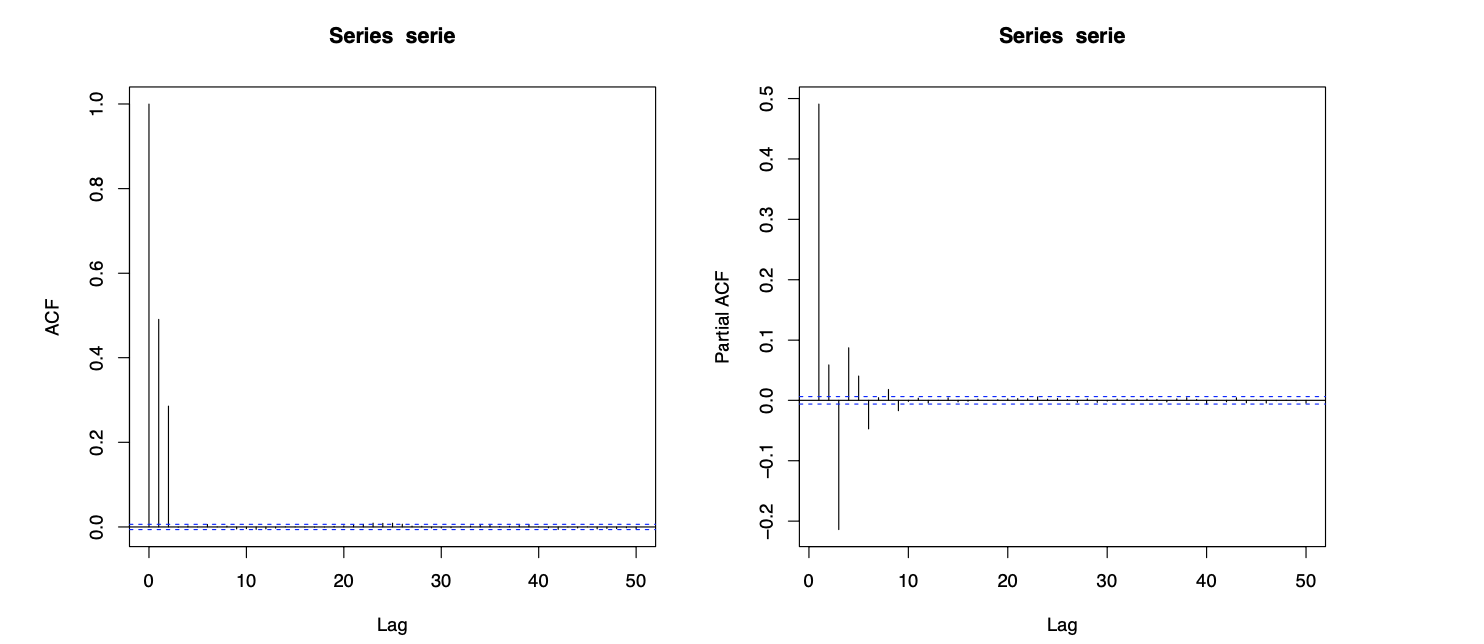
\includegraphics[scale=0.5]{figuras/fac_facp_1.png}
			
		\end{figure}
		
		\begin{enumerate}
			\item[(A)] ARMA(5,1)
			\item[(B)] AR(3) 
			\item[(C)] MA(3)
			\item[(D)] MA(2)
		\end{enumerate}
		
		\item[2] Observando a FAC e FACP, assinale qual processo é mais provável de ter gerado os dados. Justifique sua resposta.
		
		\begin{figure}[H]
			\centering 
			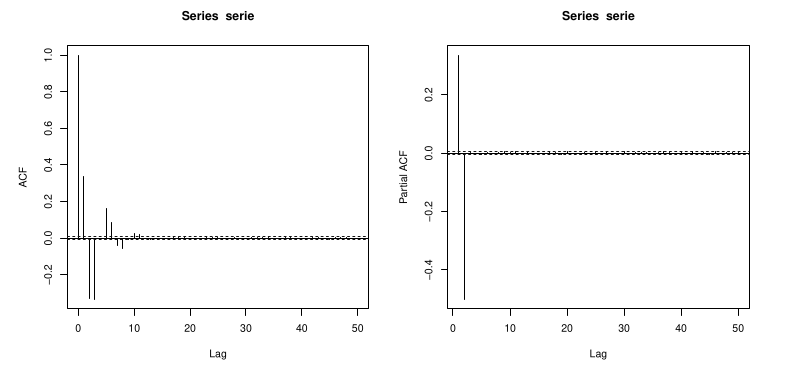
\includegraphics[scale=0.45]{figuras/fac_facp_2.png} 
		\end{figure}
		
		\begin{itemize}
			
			\item[(a)] $\mathrm{AR}(1)$
			
			\item[(b)] $\mathrm{AR}(2)$
			
			\item[(c)] $\mathrm{MA}(1)$
			
			\item[(d)] $\mathrm{MA}(2)$
			
			\item[(e)] $\operatorname{ARMA}(1,1)$
		\end{itemize}
		
		\item[3] Considere o seguinte processo estocástico estacionário:
		$$Y_t = \rho_0 Y_{t-1} + \epsilon_t\, ,$$
		onde $\epsilon_t \overset{\text{iid}}{\sim} N(0,\sigma^2_0)$, e $|\rho_0| < 1$.
		
		\begin{enumerate}
			\item[(a)] Mostre que:
			$$Y_t = \epsilon_t + \sum_{j=1}^\infty \rho^j_0 \epsilon_{t-j} \, .$$
			\item[(b)] Com base no resultado do item anterior, argumente que, para todo $t > 1$, a distribuição de $Y_t$, condicional a $Y_1, \ldots Y_{t-1}$, é Gaussiana com média $\rho_0 Y_{t-1}$ e variância $\sigma^2_0$, isto é:
			
			$$Y_t|Y_1,\ldots, Y_{t-1} \sim N(\rho_0 Y_{t-1}, \sigma^2_0)\, .$$
			\item[(c)] Com base no resultado do item anterior, e no fato de que a densidade de $Y_{2}, Y_{3},\ldots Y_{T}$, condicional a $Y_{1}$, se fatora como:
			\begin{equation*}
				\begin{aligned}	
					f_{ Y_{2},\ldots Y_{T}|Y_1}(Y_{2},Y_{3},\ldots Y_{T}|Y_1) =  \prod_{t=2}^T f_{Y_{t}|Y_1,\ldots Y_{t-1}}(Y_{t}|Y_1,\ldots Y_{t-1})  \, ;
				\end{aligned} 
			\end{equation*}
			mostre que a densidade de $Y_2,\ldots Y_T$, condicional a $Y_1$ se escreve como:
			$$f_{Y_2,\ldots, Y_T|Y_1}(Y_2,\ldots, Y_T|Y_1) = \frac{1}{\sigma^{T-1}_0}\prod_{t=2}^T\phi\left(\frac{Y_t - \rho_0 Y_{t-1}}{\sigma_0}\right)\, ,$$
			onde $\phi(x) = \frac{1}{\sqrt{2\pi}}\exp(-x^2/2)$ é a densidade de uma normal padrão.
			\item[(d)]	Mostre que o estimador $\hat{\rho}$ de $\rho_0$ que maximiza a log-verossimilhança de $Y_2,\ldots Y_T|Y_1$ é idêntico ao estimador condicional de um AR(1) visto em aula, que minimiza:	
			$$\min_{b \in \mathbb{R}}\sum_{t=2}^T (Y_t - b Y_{t-1})^2$$
		\end{enumerate}
	\end{enumerate}
	
	\paragraph{Parte 2}
	\begin{enumerate}
		\item[4] Verdadeiro ou falso? Justifique.
		
		\begin{quote}
			O critério MAIC de Ng e Perron difere do critério de informação AIC para avaliação da qualidade preditiva de um modelo, no sentido em que a medida do erro de previsão, no MAIC, é calculada sob a hipótese nula de raiz unitária, enquanto o critério AIC utiliza a soma dos quadrados dos resíduos do modelo irrestrito estimado.
		\end{quote}
		\item[5] Você é um pesquisador interessado em projetar uma série I(1) de interesse. Você decide utilizar a metodologia de Box-Jenkins como ponto de partida, e se encontra na etapa de diagnóstico dos modelos candidatos. 
		\begin{itemize}
			\item[(a)] Um de seus modelos candidatos é um ARIMA(1,1,1). Ao analisar os resíduos do modelo estimado, você se depara com o seguinte resultado:
			
			\begin{figure}[H]				
				\centering 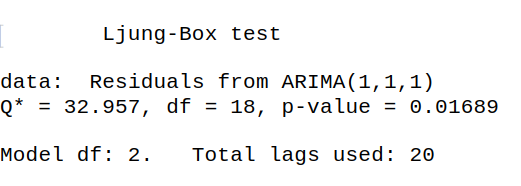
\includegraphics[scale=0.5]{figuras/lb.png}
			\end{figure}
			
			Qual é a hipótese nula do teste apresentado acima? E a alternativa? Você rejeita a nula a 5\% de significância? Quais as implicações desse resultado, em termos da qualidade preditiva do modelo estimado?
			
			\item[(b)] Você encontra um modelo que parece satisfazer os principais critérios de qualidade preditiva. No entanto, ao rodar o teste de Jarque-Bera, você encontra um $p$-valor de $0.000001$. Intrigado com o resultado, você constrói um histograma dos resíduos, sobre o qual sobrepõe a distribuição normal cuja média e variância coincidem com a dos resíduos.
			\begin{figure}[H]
				\centering
				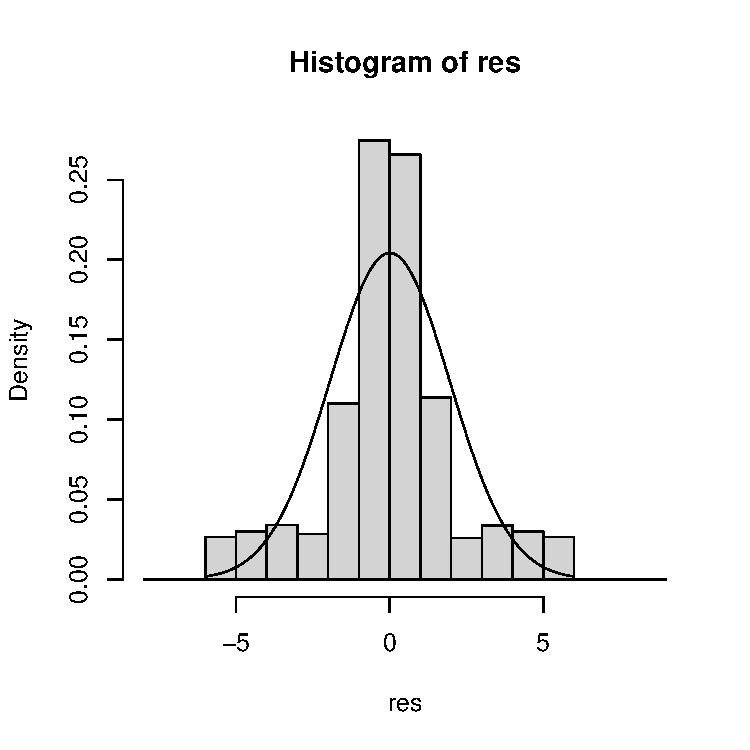
\includegraphics[scale=0.6]{figuras/jb.pdf}
			\end{figure}
			
			
			Qual é a hipótese nula do teste de Jarque-Bera? E a alternativa? A 5\% de significância, você rejeita a hipótese nula? Com base no gráfico acima, indique o motivo suspeito pelo qual você obteve a referida conclusão no teste. Quais as implicações do resultado do teste para a estimação do seu modelo?
			
		\end{itemize}
		
\item[6] Para cada uma das séries de tempo analisadas por vocês nos exercícios sobre raiz unitária.
\begin{enumerate}
	\item Divida o conjunto de dados em duas janelas, primeira em segunda, em que a primeira contém 4/5 dos períodos de tempo, e a segunda contém a quinta parte final. \textit{Dica:} use o comando \texttt{window} visto em aula.
	\item Com base na primeira janela, realize a etapa de identificação da metodologia de Box-Jenkins. Quais são os modelos candidatos? Por quê?
	\item Com base na primeira janela, estime os modelos candidatos. Com base nos critérios de diangóstico, selecione um ou mais modelos com boas métricas. Justifique suas escolhas.
	\item Compute as previsões para até um ano fora da primeira janela. Reporte os intervalos de predição associados. Como as predições se compararam ao que ocorreu na segunda janela? Qual é a interpretação do erro de previsão, nesse caso?
	\item Agora, para cada período na segunda janela, compute a previsão um passo à frente, com base nos dados até o período imediatamente anterior, para cada modelo Arima por você selecionado na primeira janela. Calcule o erro quadrático médio, um passo à frente, com base nos erros dessas previsões. Dentre os modelos por você estimados, qual se saiu melhor? Suas conclusões batem com o desempenho calculado no item anterior? Qual a diferença entre as métricas?
\end{enumerate}

	
\item[7]  Observando a FAC e FACP da série de tempo \emph{mensal} estacionária abaixo, indique qual processo SARIMA é o mais adequado de haver gerado os dados. Justifique sua resposta.

\begin{figure}[H]
	\centering
	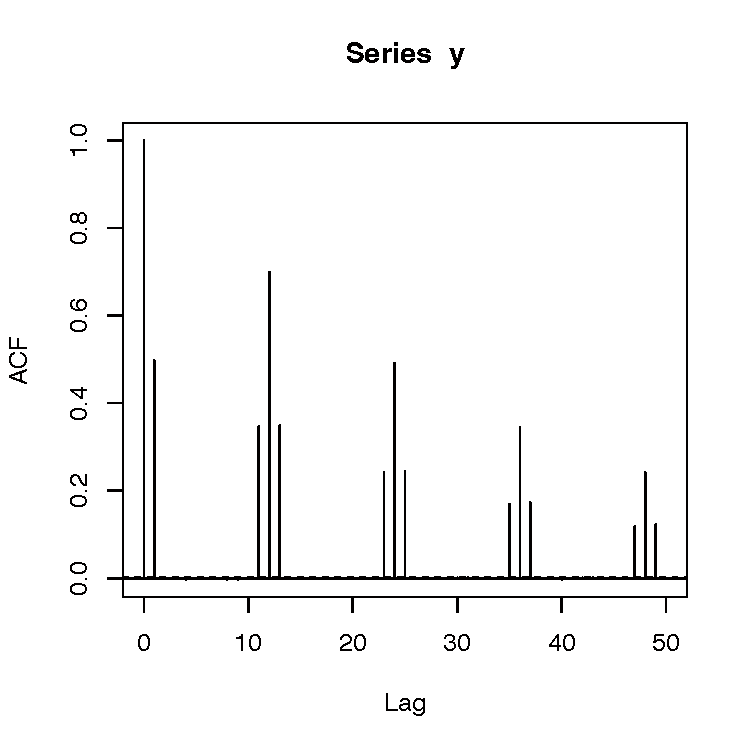
\includegraphics[scale=0.45]{acf_bw.pdf}
	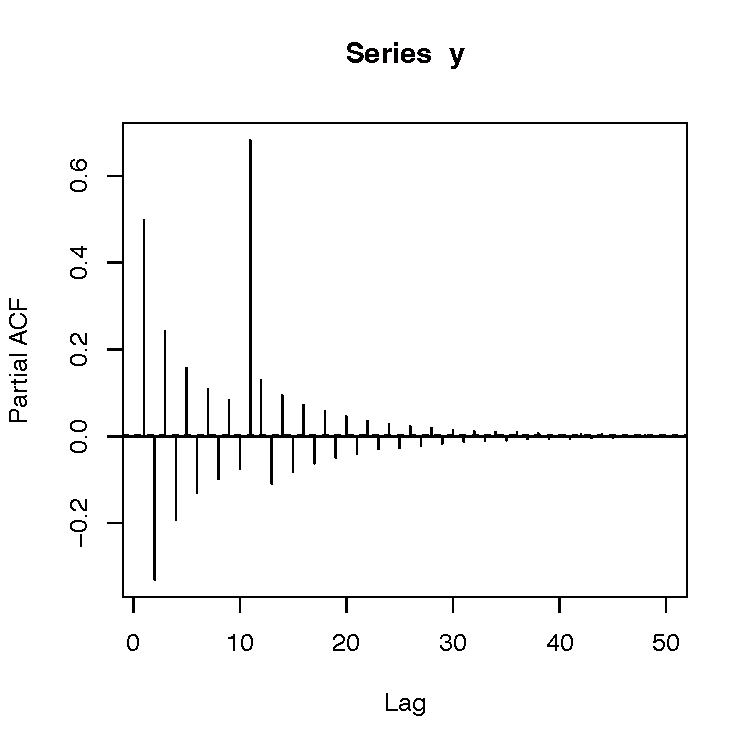
\includegraphics[scale=0.45]{pacf_bw.pdf}
\end{figure}


		\item[8] Dizemos que uma variável aleatória segue distribuição $\text{Laplace}(c,d)$ se admite densidade:

	$$f(x) = \frac{1}{2}\exp(-|x-c|/d) \, .$$
	Nesse caso, a média da variável aleatória é $c$, e sua variância é $2d^2$.

	 Mostre que o estimador de máxima verossimilhança do parâmetro $\rho_0$ de um AR(1) (sem intercepto) com ruído branco $\epsilon_t \overset{\text{iid}}{\sim}\text{Laplace}(0,d_0)$, que maximiza a log-verossimilhança da distribuição de $Y_2,\ldots, Y_T$ condicional a $Y_1$, é idêntico ao estimador $\hat \rho$ que minimiza:
	$$\min_{b \in \mathbb{R}}\sum_{t=2}^T |Y_t - b Y_{t-1}|$$
	
	
		
	

\end{enumerate}

\end{document}